% Chapter 1

\chapter{Introduction} % Main chapter title

\label{intro} % For referencing the chapter elsewhere, use \ref{Chapter1} 

\lhead{Chapter 1. \emph{Introduction}} % This is for the header on each page - perhaps a shortened title

%----------------------------------------------------------------------------------------


\section{The Standard Model of Particle Physics}

\subsection{Properties of the Standard Model}
The Standard Model (SM) of particle physics consists of a mathematical framework and physical description of all subatomic processes observed to this point.  Since its inception it has shown remarkable predictive power, although it has also been adapted over time to assimilate new measured phenomena.  The current state of the SM dates to the initial proposal that electroweak interactions could be described by an $SU(2) \times U(1)$ symmetry followed by the inception of the concept that these interactions could be described via spontaneous gauge symmetry breaking and the Higgs mechanism~\cite{StandardModelPrimer,Glashow:1961tr,PhysRevLett.13.508,Weinberg:1967tq,1964PhL....13..168S}.  The strong force was later added, including quantum chromodynamics (QCD), quark mixing angles, and the full 3-generation formulation~\cite{StandardModelPrimer,PhysRevD.2.1285,PhysRevLett.27.1688,PhysRevLett.10.531}.  The current state of the SM is a non abelian gauge theory with the symmetry group 

\begin{equation}
SU(3)_{C} \times SU(2)_{L} \times U(1)_{Y}
\label{eq:SMSymmetry}
\end{equation}

where $SU(3)_{C}$ denotes the strong QCD interaction, $SU(2)_{L}$ the weak interactions, and $U(1)_{Y}$ the electromagnetic interaction.  The generator of the $U(1)_{Y}$ group, Y, is called the hypercharge and the generator of the $SU(2)_{L}$, T, is called the weak isospin.  Right handed fermions have a weak isospin of zero, and thus do not interact via the weak force.  Before electroweak symmetry breaking there are 3 weak force bosons ($W^{+,-,3}$), one electromagnetic boson (B), and two complex scalar fields ($\phi^{+,0}$).  Electroweak symmetry breaking causes the mixing of the third weak boson and the B boson to create a neutral weak force mediator (Z) and a neutral electromagnetic force mediator ($\gamma$), and only the neutral scalar field is the only survivor of the pair becoming the Higgs boson (H).  This symmetry breaking enforces the necessary gauge invariance of $SU(2)_{L} \times U(1)_{Y}$ and gives the $W^{+,-}$ and $Z$ bosons their mass.  

Color charge is the generator of the strong QCD $SU(3)_{C}$ group, and results in eight gluon fields that are the strong force mediators.  There are three possible values of color (r,g,b) and only the quarks and the gluons have color charge, with quarks possessing one color charge and gluons possessing two.  Unlike photons, gluons can interact with themselves, but single quarks and gluons can not be isolated and thus bare color charge is not an observable quantity.   

There are 12 fermions total in the SM, six leptons and six quarks.  The leptons are divided in to three generations: Electrons and electron neutrinos ($e^{-}, \nu_{e}$, muons and muon neutrinos ($\mu^{-}, \nu_{\mu}$), and taus and tau neutrinos ($\tau, \nu_{\tau}$).  Every charged lepton has an oppositely charged anti particle, and possesses a lepton number (L) of one.  The quarks are likewise organized in a three generation scheme, each possessing pairs of quarks with electromagnetic charges of $2/3$ and $-1/3$: the up and down quarks, charm and strange, and top and bottom.  The quarks have a baryon number of $1/3$, and due to the triple-valued color charge they possess and the necessary ``colorlessness'' of the strong force they exist in either combinations of three quarks (hadrons) or quark anti-quark pairs (mesons).  Both quarks and leptons have electromagnetic charges ($Q_{em}$) dependent on their hypercharge and the third component of their weak isospin, according to the relation in~\ref{eq:ChargeRelation}.


\begin{equation}
Q_{em} = T_{3} + \frac{1}{2}Y
\label{eq:ChargeRelation}
\end{equation}

The fermions are summarized in Table~\ref{tab:FermionTable}.



\begin{table}[!Hhtbp]
\begin{tabular}{|c|cccc|cc|c|c|}
\hline
{Fermion type}  & {$Q_{em}$}& {$T_{3}$}& {$T$} &{$Y$} & {L}& {B} &{Spin} &{Color charge}\\
\hline
\hline
{$\ell_{L}$}  & {$-1$}& {$-1/2$}& \multirow{2}{*}{$1/2$} &\multirow{2}{*}{$-1$} & \multirow{2}{*}{1}& \multirow{2}{*}{0} &\multirow{2}{*}{1/2} &\multirow{2}{*}{0}\\
{$\nu_{\ell,L}$}  & {$0$}& {$1/2$}& {} &{} & {}& {} &{} &{}\\
\hline
{$\ell_{R}$}  & {$-1$}& {$0$}& {$0$} &{$-2$} & {1}& {0} &{1/2} &{0}\\
\hline
{$u_{L}$}  & {$2/3$}& {$1/2$}& \multirow{2}{*}{$1/2$} &\multirow{2}{*}{$1/3$} & \multirow{2}{*}{0}& \multirow{2}{*}{$1/3$} &\multirow{2}{*}{1/2} &\multirow{2}{*}{1}\\
{$d_{L}$}  & {$-1/3$}& {$-1/2$}& {} &{} & {}& {} &{} &{}\\
\hline
{$u_{R}$}  & {$2/3$}& \multirow{2}{*}{$0$}& \multirow{2}{*}{$0$} &{$4/3$} & \multirow{2}{*}{0}& \multirow{2}{*}{$1/3$} &\multirow{2}{*}{1/2} &\multirow{2}{*}{1}\\
{$d_{R}$}  & {$-1/3$}& {}& {} &{$-1/3$} & {}& {} &{} &{}\\
\hline


\end{tabular}
\\
\caption[The fermions and their quantum numbers]{The standard model fermions, listed with their quantum numbers.  Note that leptons and quarks are listed independent of generation, i.e.: $\ell \in \{e,\mu,\tau\}$, $u \in $ \{u,c,t\}, and $d \in $ \{d,s,b\}.~\cite{PhysRevD.86.010001,HalzenAndMartin}}
\label{tab:FermionTable}
\end{table}


The bosons, which are the force mediators described above, also follow the same relationship between charge, weak isospin, and hypercharge as the fermions.  They, however, do not possess lepton number or baryon number.  The bosons are summarized in Table~\ref{tab:BosonTable}.




\begin{table}[!Hhtbp]
\begin{tabular}{|c|cccc|cc|c|c|}
\hline
{Boson type}  & {$Q_{em}$}& {$T_{3}$}& {$T$} &{$Y$} & {L}& {B} &{Spin} &{Color charge}\\
\hline
\hline
{$W^{+}$}  & {$1$}& {$1$}& \multirow{3}{*}{$1$} &\multirow{3}{*}{$0$} & \multirow{3}{*}{0}& \multirow{3}{*}{0} &\multirow{3}{*}{1} &\multirow{3}{*}{0}\\
{$Z$}  & {$0$}& {$0$}& {} &{} & {}& {} &{} &{}\\
{$W^{-}$}  & {$-1$}& {$1$}& {} &{} & {}& {} &{} &{}\\
\hline
{$\gamma$}  & {$0$}& {$0$}& {$0$} &{$0$} & {0}& {$0$} &{1} &{0}\\
\hline
{$g$}  & {$0$}& {$0$}& {0} &{0} & {0}& {0} &{1} &{2}\\
\hline
{$H$}  & {$0$}& {$-1/2$}& {$1/2$} &{$1$} & {0}& {0} &{1} &{0}\\
\hline


\end{tabular}
\\
\caption[The bosons and their quantum numbers]{The standard model bosons, listed with their quantum numbers~\cite{PhysRevD.86.010001,HalzenAndMartin}.}
\label{tab:BosonTable}
\end{table}


The allowed interactions of the SM are depicted in Figure~\ref{figapp:SMInteractions}.  Note that leptons and quarks cannot interact with each other directly, without the ``help'' of the force mediators.


\begin{figure}[!Hh]
       \centering
       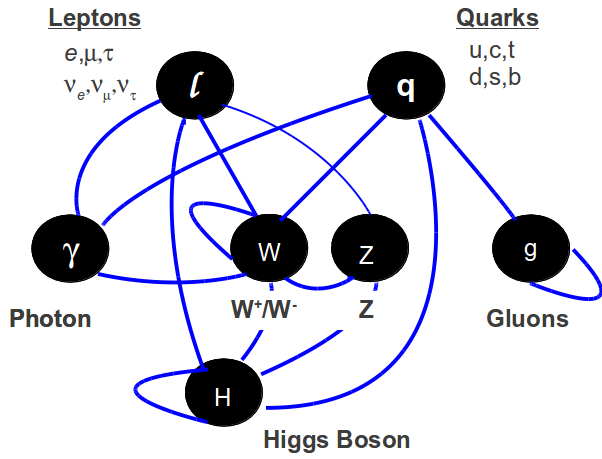
\includegraphics[scale=0.65]{Figures/SM_Interactions.png} 
       \caption[The particles of the Standard Model and their permitted interactions]{The particles of the SM depicted with all tree level permitted interactions.  The top row contains the fermions, the center row contains the force mediating bosons, and the bottom row contains the Higgs boson.}
\label{figapp:SMInteractions}
\end{figure}


\subsection{Beyond the Standard Model}

While the Standard Model has been heavily probed by experiments and proves to be a very powerful predictive tool, it does have numerous limitations.  It possesses no description of the force of gravity whatsoever, despite its considerations of every other known fundamental force.  Explanations have been attempted to account for this via the combination of principles of supersymmetry and gravity known as ``supergravity'' theories, or SUGRA.  Of those fundamental forces, the Standard Model accounts for the relative strengths of the electromagnetic, weak, and strong forces but cannot do so for the difference between the electroweak force strength and the gravitational.  This difference is known as the ``hierarchy problem'' and is also closely tied to the problem of large radiative corrections to the Higgs mass (a ``fine-tuning'' problem).  Additionally, the SM and the Higgs mechanism specifically predict massive leptons with massless neutrinos, which conflicts with the experimentally confirmed model of neutrino oscillation.  

In addition to these problems, the SM leaves open a few compelling questions.  One question, first revealed by the field of astrophysics, is that of dark matter.  Observations of rotation curves of galaxies indicated that nonluminal mass must be present.  An alternative theory of modified Newtonian dynamics was proposed, but then disproven initially by observations of the Bullet cluster and later by other similar phenomena.  The Bullet cluster data showed gravitational lensing occurring in nonluminous regions of two colliding galaxies, which made the issue of actual nonluminal matter concrete.  Measurements of the quantity of our universe that is made of dark matter indicate that it is actually the majority of all matter in our universe, and there is no mechanism in the SM that could explain that fact.  While neutrinos qualify for the qualitative properties of dark matter they cannot explain the quantity of mass that must be nonluminal, and thus there is no dark matter ``candidate'' particle present in the SM.  Numerous models beyond the SM (BSM) contain such candidates, such as supersymmetry and string theory.  Additional questions raised in astrophysics that the SM cannot explain are the observed rate of expansion and the necessary abundance of ``dark energy'' that contributes to this expansion.

Outside of the field of astrophysics the SM offers an additional question: it lacks any explanation for the symmetry between the three generations of quark pairs and the three generations of lepton pairs.  The existence of this symmetry implies a presence of a mechanism to account for it.  Numerous extensions to the SM contain such a mechanism: a hypothetical new particle that possesses both lepton and quark number.  This particle is called a leptoquark and a search for its decay signatures at the LHC is the main subject of this thesis.


\section{Leptoquarks}

\subsection{Theoretical considerations}
\label{theoreticalconsiderations}

Various extensions to the SM include predictions of new bosons that carry both lepton and baryon number, motivated by the essential symmetry of leptons and quarks in it.  Triangle anomalies that otherwise threaten the renormalizability of the SM are canceled by the requirement

\begin{equation}
\sum_{n} Q^{2}_{en} (Q_{L}-Q_{R})_{n} = 0
\label{eq:TriangleCancellation}
\end{equation}

for each of the three fermionic families, where $Q_{en}$, $Q_{Ln}$, and $Q_{Rn}$ denote the elecromagnetic, left-, and right-handed neutral current charges~\cite{Blumlein:1996qp}.  


These new bosons, called leptoquarks (LQ) are hypothetical color-triplet bosons with spin 0 (scalar LQ) or 1 (vector LQ) that are predicted by many extensions of the
standard model (SM) of particle physics, such as Grand Unified Theories~\cite{PhysRevLett.32.438,Pati:1973uk,Pati:1974yy,Murayama:1991ah,Fritzsch:1974nn,Senjanovic:1982ex,PhysRevLett.65.2209,Frampton:1990hz}, technicolor schemes~\cite{Dimopoulos:1979es,Dimopoulos:1979sp,Farhi:1980xs}, and composite models~\cite{Schrempp:1984nj}. They carry fractional electric charge ($\pm \frac{1}{3}$ for LQs considered in this paper) and both baryon and lepton numbers and thus couple to a lepton
and a quark.  Existing experimental
limits on flavor changing neutral currents and other
rare processes disfavor leptoquarks that couple to a quark and lepton of a different SM generation or of more than one SM generation~\cite{Buchmuller:1986iq,FCNC}.  

The description of the LQ phenomenology considered in this thesis begins with an effective lagrangian put forth by W. Buchmuller, R. Ruckl, and D. Wyler in 1986 in the lead up to the turning on of the HERA collider.  ~\cite{Belyaev:2005ew,Buchmuller:1986zs} with the general dimensionless SU(3) $\times$ SU(2) $\times$ U(1) invariant couplings of scalar and vector leptoquarks to leptons and quarks, satisfying baryon and lepton number conservation:


\begin{equation}
\mathcal{L} = \mathcal{L}^{f}_{|\text{F}|=0} + \mathcal{L}^{f}_{|\text{F}|=2}
\label{eq:LQsmalllagrangian}
\end{equation}

The $\mathcal{L}^{f}_{|\text{F}|=0,2}$ Lagrangians describe the Yukawa interactions of LQs with leptons and quarks, changing the fermion number $F$ by 0 or 2, where $F=3B+L$, $B$ is the baryon number and $L$ is the leptons number.  $\mathcal{L}^{f}_{|\text{F}|=0,2}$ are diagonal in flavor:


%%Note: In the paper by S. Belyaev, S and R are both scalar and V and U are both vector
%Also, rather than subscripts denoting the weak isospin, subscripts denote the *dimension* of the weak isospin represatation, thus, following:
% N= 2*I+1
% We have 0->1, 1/2->1, 1->3 to convert from this subscript to S. Belyaev's

\begin{eqnarray}
\mathcal{L}^{f}_{|\text{F}|=0} &=& (h_{2L}\bar{u}_{R}\ell_{L}+h_{2R}\bar{q}_{L}i\sigma_{2}e_{R})S_{\frac{1}{2}} +\tilde{h}_{2L}\bar{d}_{R}\ell_{L}\tilde{S_{\frac{1}{2}}} \nonumber\\
&& +(h_{1L}\bar{q}_{L}\ell_{L}+h_{1R}\bar{d}_{R}\gamma^{\mu}e_{R})V_{0\mu} +\tilde{h}_{1R}\bar{u}_{R}\gamma^{\mu}e_{R}\tilde{V}_{0\mu} \nonumber\\
&&+h_{3L}\bar{q}_{L}\vec{\sigma}\gamma^{\mu}\ell_{L}\vec{V}_{1\mu} +h.c.
\label{eq:LQlagrangianF0},
\end{eqnarray}


\begin{eqnarray}
\mathcal{L}^{f}_{|\text{F}|=2} &=& (g_{2L}\bar{d}^{c}_{R}\gamma^{\mu}\ell_{L}+g_{2R}\bar{q}^{c}_{L}\gamma^{\mu}e_{R})V_{\frac{1}{2}\mu} + \tilde{g}_{2L}\bar{u}^{c}_{R}\gamma^{\mu}\ell_{L}\tilde{V}_{\frac{1}{2}\mu} \nonumber \\
&& +(g_{1L}\bar{q}^{c}_{L}i\sigma_{2}\ell_{L}+g_{1R}\bar{u}^c_{R}e_{R})S_{0}+\tilde{g}_{1R}\bar{d}^c_{R}e_{R}\tilde{S}_{0}  \nonumber \\
&& +g_{3L}\bar{q}^{c}_{L}i\sigma_{2}\vec{\sigma}\ell_{L}\vec{S}_{1} +h.c.
\label{eq:LQlagrangianF2},
\end{eqnarray}

where $q_L$ and $\ell_L$ are the left handed quark and lepton SU(2) doublets, and $e_R$, $d_R$, $u_R$ are the right handed charged leptons, down-, and up-quarks, respectively.  Charge conjugated fields are denoted by $\psi_c=\bar{\psi}^T$, $\sigma_i$ are the Pauli spin matrices.  The subscripts L, R, of the coupling constants $g_{i}$ and $h_{i}$ denote the lepton chirality.  The LQ indices give the weak isospin.  



\begin{table}[!Hhtbp]
\begin{tabular}{|c|ccccc|ccc|c|}
\hline
{LQ type}  & {$Q_{em}$}& {$T_{3}$}& {$T$} &{$Y$}& {F=3B+L}& {$\lambda_{L}(\ell q)$}& {$\lambda_{L}(\nu q)$}& {$\lambda_{R}(\ell q)$}&{Final States}\\
\hline
\hline
{$S_{0,L}$}  & {$1/3$}& {$0$}& {$0$} &{$2/3$}& {$-2$}& {$g_{1L}$}& {$-g_{1L}$}& {$0$}&{$\ell^{+}_{L}\bar{u}_{L},\bar{\nu}_{L}\bar{d}_{L}$}\\
\hline
{$S_{0,R}$}  & {$1/3$}& {$0$}& {$0$} &{$2/3$}& {$-2$}& {$0$}& {$0$}& {$g_{1R}$}&{$\ell^{+}_{R}\bar{u}_{R}$}\\
\hline
{$\tilde{S}_{0,R}$}  & {$4/3$}& {$0$}& {$0$} &{$8/3$}& {$-2$}& {$0$}& {$0$}& {$\tilde{g}_{1R}$}&{$\ell^{+}_{R}\bar{d}_{R}$}\\
\hline
{$S_{\frac{1}{2},L}$}  & {$5/3$}& {$1/2$} & \multirow{2}{*}{$1/2$}&\multirow{2}{*}{$7/3$}& \multirow{2}{*}{$-2$}& {$h_{2L}$}& {$0$}& {$0$}&{$\ell^{+}_{L}u_{L}$}\\
{$S_{\frac{1}{2},L}$}  & {$2/3$}& {$-1/2$} & {}&{}& {}& {$0$}& {$h_{2L}$}& {$0$}&{$\bar{\nu}_{L}u_{L}$}\\
\hline
{$S_{\frac{1}{2},R}$}  & {$5/3$}& {$1/2$} & \multirow{2}{*}{$1/2$}&\multirow{2}{*}{$7/3$}& \multirow{2}{*}{$-2$}& {$0$}& {$0$}& {$h_{2R}$}&{$\ell^{+}_{R}u_{R}$}\\
{$S_{\frac{1}{2},R}$}  & {$2/3$}& {$-1/2$} & {}&{}& {}& {$0$}& {$0$}& {$-h_{2R}$}&{$\ell^{+}_{R}d_{R}$}\\
\hline
{$\tilde{S}_{\frac{1}{2},L}$}  & {$2/3$}& {$1/2$} & \multirow{2}{*}{$1/2$}&\multirow{2}{*}{$1/3$}& \multirow{2}{*}{$-2$}& {$\tilde{h}_{2L}$}& {$0$}& {$0$}&{$\ell^{+}_{L}d_{L}$}\\
{$\tilde{S}_{\frac{1}{2},L}$}  & {$-1/3$}& {$-1/2$} & {}&{}& {}& {$0$}& {$\tilde{h}_{2L}$}& {$0$}&{$\bar{\nu}_{L}d_{L}$}\\
\hline
{$S_{1,L}$}  &{$4/3$}& {$1$} & \multirow{3}{*}{$1$}&\multirow{3}{*}{$2/3$}& \multirow{3}{*}{$-2$}& {$-\sqrt{2}g_{3L}$}& {$0$}& {$0$}&{$\ell^{+}_{L}\bar{d}_{L}$}\\
{$S_{1,L}$}  &{$1/3$}& {$0$} &&&& {$-g_{3L}$}& {$0$}& {$-g_{3L}$}&{$\ell^{+}_{L}\bar{u}_{L},\bar{\nu}_{L}\bar{d}_{L}$}\\
{$S_{1,L}$}  &{$-2/3$}& {$-1$} &&&& {$$}& {$0$}& {$\sqrt{2}g_{3L}$}&{$\bar{\nu}_{L}\bar{u}_{L}$}\\

\hline
\hline
{$V_{0,L}$}  & {$2/3$}& {$0$}& {$0$} &{$4/3$}& {$-2$}& {$h_{1L}$}& {$h_{1L}$}& {$0$}&{$\ell^{+}_{L}d_{R},\bar{\nu}_{L}u_{R}$}\\
\hline
{$V_{0,R}$}  & {$2/3$}& {$0$}& {$0$} &{$4/3$}& {$-2$}& {$0$}& {$0$}& {$h_{1R}$}&{$\ell^{+}_{R}d_{L}$}\\
\hline
{$\tilde{V}_{0,R}$}  & {$5/3$}& {$0$}& {$0$} &{$10/3$}& {$-2$}& {$0$}& {$0$}& {$\tilde{h}_{1R}$}&{$\ell^{+}_{R}u_{L}$} \\
\hline
{$V_{\frac{1}{2},L}$}  & {$4/3$}& {$1/2$} & \multirow{2}{*}{$1/2$}&\multirow{2}{*}{$5/3$}& \multirow{2}{*}{$-2$}& {$g_{2L}$}& {$0$}& {$0$}&{$\ell^{+}_{L}\bar{d}_{R}$}\\
{$V_{\frac{1}{2},L}$}  & {$1/3$}& {$-1/2$} & {}&{}& {}& {$0$}& {$g_{2L}$}& {$0$}&{$\bar{\nu}_{L}\bar{d}_{R}$}\\
\hline
{$V_{\frac{1}{2},R}$}  & {$4/3$}& {$1/2$} & \multirow{2}{*}{$1/2$}&\multirow{2}{*}{$5/3$}& \multirow{2}{*}{$-2$}& {$0$}& {$0$}& {$g_{2R}$}&{$\ell^{+}_{R}\bar{d}_{L}$}\\
{$V_{\frac{1}{2},R}$}  & {$1/3$}& {$-1/2$} & {}&{}& {}& {$0$}& {$0$}& {$g_{2R}$}&{$\ell^{+}_{R}\bar{u}_{L}$}\\
\hline
{$\tilde{V}_{\frac{1}{2},L}$}  & {$1/3$}& {$1/2$} & \multirow{2}{*}{$1/2$}&\multirow{2}{*}{$-1/3$}& \multirow{2}{*}{$-2$}& {$\tilde{g}_{2L}$}& {$0$}& {$0$}&{$\ell^{+}_{L}\bar{u}_{R}$}\\
{$\tilde{V}_{\frac{1}{2},L}$}  & {$-2/3$}& {$-1/2$} & {}&{}& {}& {$0$}& {$\tilde{g}_{2L}$}& {$0$}&{$\bar{\nu_{L}}\bar{u}_{R}$}\\
\hline
{$V_{1,L}$}  &{$5/3$}& {$1$} & \multirow{3}{*}{$1$}&\multirow{3}{*}{$4/3$}& \multirow{3}{*}{$-2$}& {$\sqrt{2}h_{3L}$}& {$0$}& {$0$}&{$\ell^{+}_{L}u_{R}$}\\
{$V_{1,L}$}  &{$2/3$}& {$0$} &&&& {$-h_{3L}$}& {$0$}& {$h_{3L}$}&{$\ell^{+}_{L}\bar{d}_{R},\bar{\nu}_{L}u_{R}$}\\
{$V_{1,L}$}  &{$-1/3$}& {$-1$} &&&& {$$}& {$0$}& {$\sqrt{2}h_{3L}$}&{$\bar{\nu}_{L}d_{R}$}\\

\hline


\end{tabular}
\\
\caption[The types of scalar and vector LQs with their quantum numbers, coupling strenths, and final state decay modes]{Scalar (S) and vector (V) type LQs, with their quantum numbers, coupling strengths, and final state decay modes.  Quantum numbers given are fermion number (F), hypercharge (Y), weak isospin ($T$), the third component of weak isospin ($T_{3}$), and electric charge ($Q_{em}$).}
\label{tab:LQTable}
\end{table}


\subsection{Signatures at the LHC}
In pp collisions LQs can be produced either singly or in pairs, with very similar final state decay products.  In pair production, LQs are produced predominantly via gluon-gluon fusion with additional contributions from quark-quark annihilation, as indicated in Eq.~\ref{eq:PairLQ1} and Eq.~\ref{eq:PairLQ2}


\begin{equation}
g+g\rightarrow \text{LQ}+\overline{\text{LQ}}
\label{eq:PairLQ1}
\end{equation}



\begin{equation}
q+\overline{q}\rightarrow \text{LQ}+\overline{\text{LQ}}
\label{eq:PairLQ2}
\end{equation}

These decay modes result in a final state of two leptons and two jets.  Single production of LQs occurs in association with a lepton via quark-gluon fusion, as indicated in Eq.~\ref{eq:SingleLQ1}, and thus results in a final state of two leptons and one jet.



\begin{equation}
q+g\rightarrow \text{LQ}+\ell
\label{eq:SingleLQ1}
\end{equation}

Of all the diagrams contributing to pair production, only one posseses any $\lambda$-dependance at all and the overall dependence on $\lambda$ in pair production is negligible~\cite{Hewett:1997ce}.  In contrast to this single production diagrams, depicted in Figures~\ref{figapp:schanneldiag} through~\ref{figapp:tchannel2diag}, do scale with the coupling.  Single production cross sections decrease more slowly with the coupling, exceeding pair production at an order of 1 TeV for $\lambda = 0.6$.  


\begin{figure}[!Hh]
       \centering
       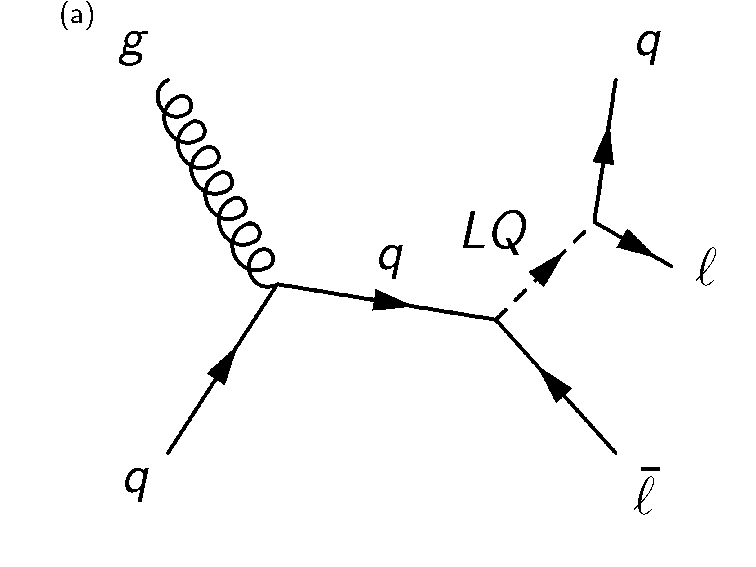
\includegraphics[scale=0.65]{Figures/schannel.pdf} 
       \caption[The $s$-channel resonant LQ production diagram.]{The $s$-channel resonant LQ production diagram.}
\label{figapp:schanneldiag}
\end{figure}


\begin{figure}[!Hh]
       \centering
       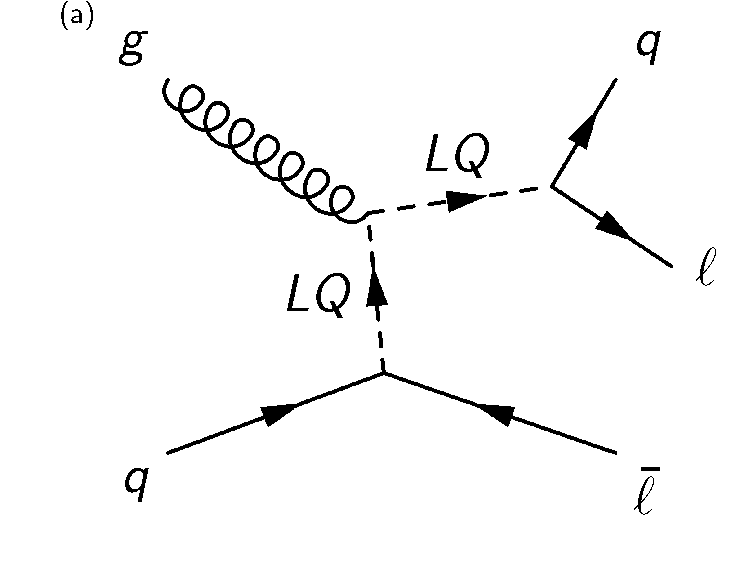
\includegraphics[scale=0.65]{Figures/tchannel1.pdf} 
       \caption[The $t$-channel LQ production diagram with a resonant production component.]{The $t$-channel LQ production diagram with a resonant production component.}
\label{figapp:tchannel1diag}
\end{figure}


\begin{figure}[!Hh]
       \centering
       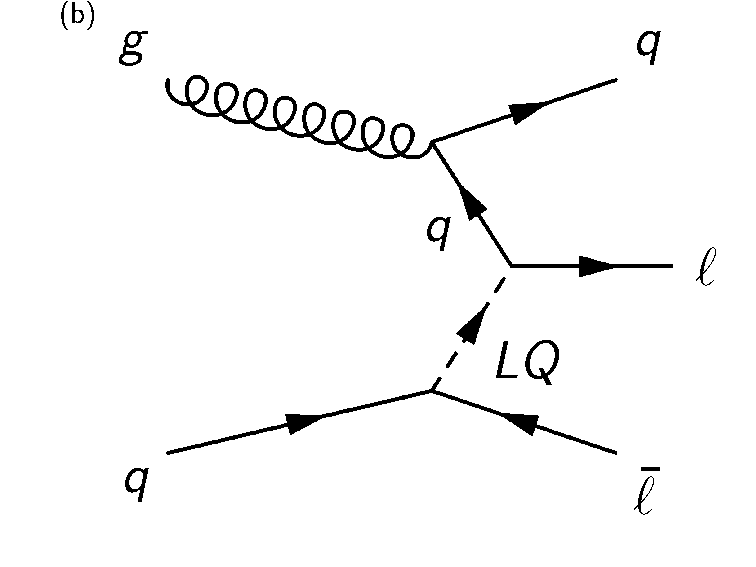
\includegraphics[scale=0.65]{Figures/tchannel2.pdf} 
       \caption[The $t$-channel nonresonant LQ production diagram.]{The $t$-channel nonresonant LQ production diagram.}
\label{figapp:tchannel2diag}
\end{figure}

The main single leptoquark production mode at the LHC is the resonant diagram shown in
Figure~\ref{figapp:schanneldiag}. However, significant contributions are made by the diagrams with non-resonant com-
ponents shown in Figures~\ref{figapp:tchannel1diag} and~\ref{figapp:tchannel2diag}. These contributions increase with both the LQ mass and coupling;
the invariant mass distribution of a first generation LQ, of LQ mass $M_{\text{LQ}}$ = 1 TeV and coupling
$\lambda$ = 1.0, possesses a tail that extends to very low masses that is comparable to the peak in
magnitude.  

Due to the parton distribution function dependence of single LQ production, the cross sections for second generation LQs is significantly suppressed with respect to first generation LQs.  

The signatures for LQ single production include three-object final states with leptons ($\ell$), neutrinos ($\nu$), and a single jet ($j$).  There are two distinct final state signatures, $\ell^{+} \ell^{-} j$ and $\nu \nu j$.  This thesis considers single LQ production with $\beta=1.0$, thus only final state signatures with two leptons and a jet.  The major SM backgrounds that can mimic this signature are Z boson production in association with one or more jets and $t\bar{t}$ production.  In the case of Z boson production, the Z decays to two leptons yielding the same final state particles as single LQ production.  There are three possible decay modes for $t\bar{t}$ production: fully leptonic, partially leptonic, and hadronic.  It is the fully leptonic mode, $t\bar{t} \rightarrow bW(\rightarrow\ell\nu)bW(\rightarrow\ell\nu)$ that can mimic single LQ production with two charged leptons, although it does also possess additional missing transverse energy from the neutrinos.  Other SM processes that are additional small contributions to the total background that of events with two charged leptons and at least one jet are diboson (WW, WZ,ZZ) production, single t-quark production, and QCD multijet production in which two jets are misidentified as leptons.  



\subsection{Previous searches}

In addition to the indirect limits that restrict LQs to coupling to same-generation leptons discussed in Section~\ref{theoreticalconsiderations}, various collaborations have performed direct searches for LQs.  

Early searches for scalar leptoquarks were conducted at the HERA $ep$ collider by the H1~\cite{Aid:1995wd,Abt:1993nr,Collaboration:2011qaa} and ZEUS~\cite{Derrick:1993by} collaborations and found no evidence for leptoquarks.  Limits were set at 95\% confidence level of $M_{\text{LQ}}(\text{1st gen.}) < 250$ GeV for $|F|=0$ with the assumption that $\lambda > \lambda_{em}$.  Later results in 1997 from the HERA collider had intriguing implications for leptoquarks and increased interest in searches for them.  Both the H1 and ZEUS collaborations reported excesses in neutral current deep inelastic scattering events ($e^+ p \rightarrow e^+ X$) at high values of $Q^2$, where $Q^2$ is the four-momentum transfer~\cite{H1excess,ZEUSexcess}.  Figure~\ref{figapp:Q2excess} depicts the excess measured by the H1 collaboration, showing both the total number of events measured and the ratio to the SM expectation versus $Q^2$.  The reconstructed invariant mass of the final state electron and jet is compared to the SM expectation in Figure~\ref{figapp:Q2excess} with an excess visible at high values of $Q^2$, concentrated near values of $M_{e^+ j}$ of 200 GeV.  

Searches for LQs following the observation of this excess have ruled out LQs at various detectors.  The D$0$ collaboration produced limits on singly first generation LQs of $M_{\text{LQ}} > 274$ GeV ($\lambda=1.0$ and $\beta=1.0$) ~\cite{Abazov:2006ej}.  In 2011, the H1 collaboration published comprehensive limits on singly produced LQs of various types as a function of $\lambda$~\cite{Collaboration:2011qaa}, placing a limit on the $S^{R}_{0}$ type LQ that this thesis primarily considers of  $M_{\text{LQ}} > 500$ GeV ($\lambda=1.0$ and $\beta=1.0$).  These limits are shown in Figure~\ref{figapp:H1limits}.  


\textcolor{red}{FIXME: 2012 CMS results.}  %Data being collected at this very moment at a center of mass energy of 13 TeV comprise data collected on collisions at the highest energies performed to this date.  This increase in energy roughly doubles the single LQ production cross sections at the LHC, allowing for greater reach for this statistically limited search.

The 20 $fb^{-1}$ of data collected by CMS with a center-of-mass energy of $\sqrt{s}=8$\TeV is unprecedented for hadron colliders, both with respect to total integrated luminosity and collision energy.  For a statistically limited search such as the search for single LQ production, this provides significantly greater reach than achieved in the past at other colliders.  Additionally, advances in detector technology, described in Chapter 2, and in reconstruction, described in Chaper 3, provide the ability to even more precisely measure particle kinematics.  These techniques along with the increase in integrated luminosity also create a reduction of the systematic uncertainties associated with measurements made with the CMS detector.  

In this thesis, a search for single production of first- and second-generation scalar LQs with the CMS detector is presented, as a function of LQ mass and coupling $\lambda$, using all the 8 TeV collision data collected.  The SM backgrounds are studied in detail, and data-driven methods for estimating the most significant backgroudns are utilized.  


\begin{figure}[!Hh]
       \centering
       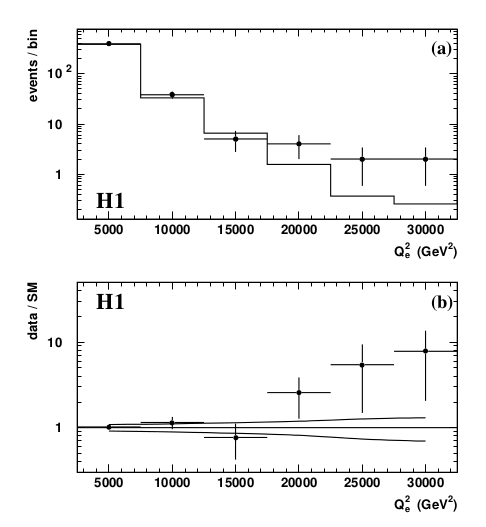
\includegraphics[scale=0.65]{Figures/H1Excess_Q2.png} 
       \caption[Excesses measured by the H1 collaboration in the $Q^2$ distribution of neutral current deep inelastic scattering events]{Observation of an excess of high $Q_e^2$ events measured by the H1 collaboration, where the subscript $e$ represents the ``e-method'' used to compute $Q^2$, using only information from the scattered electron~\cite{H1excess}.  The number of events is shown in (a), with the solid black circles representing data and the solid black line representing the neutral current deep inelastic scattering expectation.  The ratio of data over expectation is shown in (b), with the lines above and below unity representing the $\pm1\sigma$ levels calculated including both statistical and systematic errors of the expected values.}
\label{figapp:Q2excess}
\end{figure}


\begin{figure}[!Hh]
       \centering
       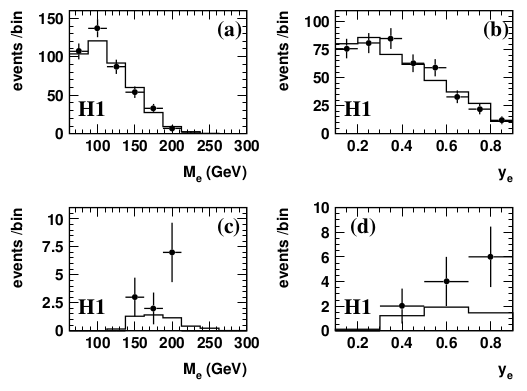
\includegraphics[scale=0.85]{Figures/H1Excess_M.png} 
       \caption[Excesses measured by the H1 collaboration in the mass and $y$ distributions of neutral current deep inelastic scattering events]{Obseravtion of an excess in the $M_e$ distribution at high values of $Q_e^2$.  The subscript $e$ represents the ``e-method'' used to compute $Q^2$, using only information from the scattered electron~\cite{H1excess}.  Distributions of $M_e$ and $y_e$ (where $y_e$ is the the ratio of the electron four momentum over the jet four-momentum) of events with $2500 \text{GeV} < Q_e^2 < 15000 \text{GeV}$ are shown in (a) and (b), respectively.  The same distributions for $Q_e^2 > 15000 \text{GeV}$ are shown in (c) and (d).}
\label{figapp:Q2excess}
\end{figure}




\begin{figure}[!Hh]
       \centering
       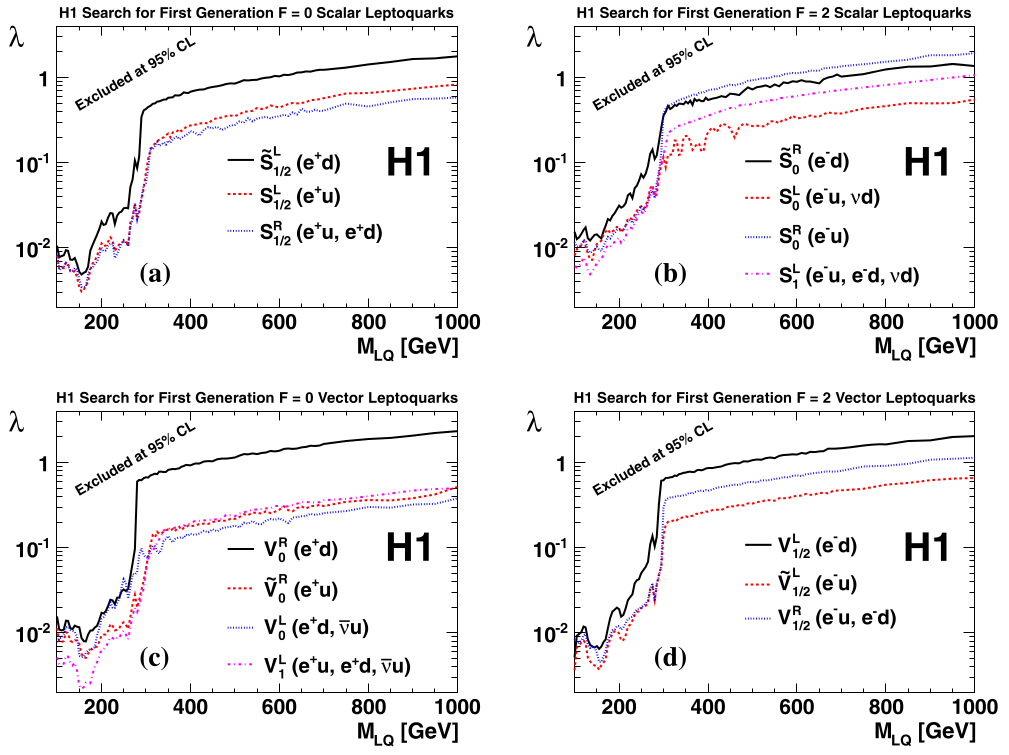
\includegraphics[scale=0.45]{Figures/H1limits.png} 
       \caption[Observed limits on LQs produced by the H1 collaboration]{Exclusion limits produced by the H1 collaboration, for all 14 LQ types as described by the LQ model in Section \label{theoreticalconsiderations}.  The limits are expressed on $\lambda$ as a function of LQ mass, for scalar LQs with F = 0 (a) and F = 2 (b) as well as for vector LQs with F = 0 (c) and F = 2 (d).  The domains above the curves are excluded at 95\% confidence level.}
\label{figapp:H1limits}
\end{figure}
